\RequirePackage{xcolor}
\documentclass[a0]{sciposter} % papersize
\usepackage{multicol,subfig,amsmath}
\usepackage{graphicx,url,hyperref,doi}
\hypersetup{hidelinks} 
%usepackage[french]{babel}   
\usepackage[utf8]{inputenc}
\usepackage[sort&compress,numbers]{natbib}
\usepackage{tikz}
\usepackage{lipsum} % filler text

% if you have your own latex installation, you need to install packages
\usepackage{algorithm} 
\usepackage{algpseudocode} 

\usepackage{listings}
\usepackage[font=small,labelfont=bf]{caption}
\tikzstyle{elem} = [draw, rectangle, thick, minimum height=2em, minimum width=2em]
\tikzstyle{line} = [draw, thick, -stealth, shorten >=1pt]
\setlength{\parskip}{3pt}
\renewcommand{\arraystretch}{1.5}

\title{Project title}
\author{Author name}
\institute{Author affiliation}
\email{student.author@email.mcgill.ca}

\leftlogo[1]{logo1.png} 
\rightlogo[1]{logo2.png}

\definecolor{codegreen}{rgb}{0,0.6,0}
\definecolor{codegray}{rgb}{0.5,0.5,0.5}
\definecolor{codepurple}{rgb}{0.58,0,0.82}
\definecolor{backcolour}{rgb}{0.95,0.95,0.92}

\lstdefinestyle{pys}{
    backgroundcolor=\color{white},   
    commentstyle=\color{codegreen},
    keywordstyle=\bfseries\color{blue},
    numberstyle=\tiny\color{codegray},
    stringstyle=\color{codepurple},
    basicstyle=\ttfamily\normalsize,
    breakatwhitespace=false,         
    breaklines=true,                 
    captionpos=b,                    
    keepspaces=true,                 
    numbers=left,                    
    numbersep=25pt,                  
    showspaces=false,                
    showstringspaces=false,
    showtabs=true,                  
    tabsize=2
}
\renewcommand*{\lstlistingname}{Code snippet}
\lstset{style=pys}

\usepackage{qrcode}

\begin{document}

% QR y nuevo logo
\conference{\raisebox{3cm}[0cm]{\qrcode[height=75mm]{https://mcgill.ca}}
  \hfill
  \raisebox{4cm}[0cm]{a QR code to the code repository would be super neat to have}
  \hfill
  \raisebox{2cm}[0cm]{\includegraphics[width=130mm]{logo3.png}}}

\maketitle
\begin{abstract}
A very brief summary
\end{abstract}

\begin{multicols}{2} 

\section{Introduction}

Avoid long sentences.

\lipsum[2-4]

\section{Background}

Be visual \citet{ai} and use
\begin{itemize}
\item bullet
\item points
\item when useful.
\end{itemize}

You can use some equations, too:
\begin{equation}
    f(x) = \sum_{i = 0}^\infty \sin(i x).
    \label{summation}
\end{equation}
Remember to discuss them to connect them to the rest of the content
and reference Equation \eqref{summation}.

\section{Methodology}

Prefer diagrams.

\begin{figure}
\captionsetup{type=figure} % for sciposter
\setcounter{figure}{0} % for sciposter
\begin{center}
    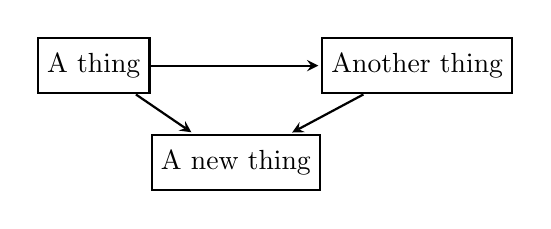
\begin{tikzpicture}[]
      \matrix[row sep=0.5cm]{
      \node[elem] (n1) {A thing}; & & \node[elem] (n2) {Another thing}; \\
      & \node[elem] (n3) {A new thing}; & \\
      };
     \draw [line] (n1) -- (n2);
     \draw [line] (n1) -- (n3);
     \draw [line] (n2) -- (n3);
    \end{tikzpicture}
\end{center}
\caption{Explain your notation.}
\label{diag}
\end{figure}

\lipsum[2]

You can also use {\em pseudocode}:

\begin{algorithmic}[1]
\State $x \leftarrow 0$
\For {$i \in [1,2,\ldots, n]$}
	\State $x \leftarrow x + i$
\EndFor
\If {$x < \beta$}
    \State $d \leftarrow \top$
\EndIf
\end{algorithmic} 

You can also throw in code if you want. Just make it small snippets
that have a clear purpose.
\begin{lstlisting}[language=Python, caption=Cool beans]
import numpy as np
from numpy.random import uniform
X = uniform(size = (3, 5))
print(np.shape(X))
\end{lstlisting}

\section{Evaluation}

Again, prefer tables and figures over text.

\lipsum[3]

\begin{figure}
\setcounter{figure}{1} 
\captionsetup{type=figure} 
\begin{center}
% From https://tex.stackexchange.com/questions/162648/how-to-draw-a-sinewave-in-tikz
  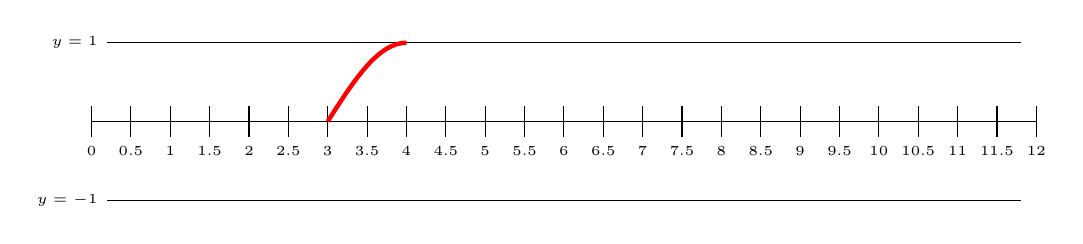
\begin{tikzpicture}
    \draw (0,0) -- (12,0);
    \draw (0.2,1)node[left,font=\tiny] {$y=1$} -- (11.8,1);
    \draw (0.2,-1)node[left,font=\tiny] {$y=-1$} -- (11.8,-1); 
    \foreach \x in {0,0.5,...,12}{
      \draw (\x,-0.2)node [below,font=\tiny,] {\x} -- (\x,0.2) ;
    }
    \draw[ultra thick, red] (3,0) sin (4,1);  
  \end{tikzpicture}
  
\end{center}
\caption{Explain how to read it.}
\label{curvas}
\end{figure}

\lipsum[1]

\begin{table}
\setcounter{table}{0} 
\captionsetup{type=table} 
\caption{Explain the notation.}
\label{data}
\begin{center}
\scalebox{0.9}{\begin{tabular}{|r|c|l|}
    \hline
         \multicolumn{1}{|c|}{\rotatebox{90}{\bf Value}}
         & \multicolumn{1}{|c|}{\rotatebox{90}{\bf Parameter}}
         & \multicolumn{1}{|c|}{\rotatebox{90}{\bf Description\phantom{m}}} \\
         \hline
         0.23 & $x$ & something \\
         \hline
         2.34 & $y$ & demonstration \\
        \hline
    \end{tabular}}
\end{center}
\end{table}

\section{Conclusions}

Highlights.

\lipsum[4]

\subsection*{Acknowledgments}

Thank people, funds, and tools.

\lipsum[1]

\end{multicols}

\bibliography{refs}
\bibliographystyle{plainnat}

\end{document}
